\chapter{Design}

Il progetto è stato guidato da un modello iterativo basato sullo \textbf{User Centered Design}.
%
Inizialmente, sono stati definiti gli utenti target dell'applicazione, sui quali sono state create le \textit{Personas}.
%
Queste ultime hanno svolto un ruolo cruciale nello sviluppo e nella comprensione delle funzionalità del sistema, garantendo un adattamento ai requisiti degli utenti.

Come processo di sviluppo abbiamo adottato una metodologia simile all'Agile, in cui sono state frequentemente analizzate le attività da svolgere e le relative priorità, così come il carico di lavoro assegnato e i feedback sul lavoro svolto.
%
Lato frontend, le interfacce utente sono state progettate secondo i principi fondamentali del design:

\begin{itemize}
    \item il \textbf{KISS} (Keep It Simple, Stupid) per garantire un'esperienza priva di complicazioni e ridurre al minimo gli errori degli utenti durante la navigazione nell'applicazione.
    \item Sono stati impiegati i principi del Responsive Design come base per garantire un elevato livello di usabilità dell'applicazione.
\end{itemize}

%
%
%
\section{Target User Analisys}

Nel processo di progettazione del nostro sistema, abbiamo identificato diversi profili di utenti per comprendere meglio le esigenze e i comportamenti dei potenziali fruitori del nostro servizio.

%
%
%
\subsection{Personas 1: Il Gamer}

\textbf{Nome:} Luca

\textbf{Età:} 23

\textbf{Occupazione:} Studente universitario e appassionato di videogiochi

\textbf{Obiettivi e Comportamenti:} Luca è un giocatore accanito che trascorre molte ore al giorno giocando a una varietà di giochi online. Cerca una piattaforma come la nostra per connettersi con altri giocatori, formare squadre e partecipare a sessioni di gioco cooperative. È interessato a funzionalità quali chat vocali durante il gioco, organizzazione di eventi e discussioni sui giochi più popolari. La sua priorità è un'interfaccia semplice e reattiva per facilitare la sua partecipazione e l'organizzazione di eventi di gioco.

%
%
%
\textbf{Personas 2: Elisa - L'appassionata di Lettura e Libri}

\textbf{Età:} 35

\textbf{Occupazione:} Libraia e Blogger

\textbf{Obiettivi e Comportamenti:} Elisa è appassionata di libri e gestisce un blog letterario. Cerca una piattaforma per connettersi con altri lettori, organizzare club del libro online e discutere di opere letterarie. Desidera una piattaforma con chat testuali, possibilità di creare gruppi tematici dedicati ai diversi generi letterari e strumenti per organizzare eventi come letture collettive e sessioni di discussione.

%
%
%
\subsection{Personas 3: Lo Studente Organizzato}

\textbf{Nome:} Giada

\textbf{Età:} 19

\textbf{Occupazione:} Studentessa universitaria

\textbf{Obiettivi e Comportamenti:} Giada è una studente impegnata che cerca un'interfaccia per connettersi con altri studenti, partecipare a discussioni relative ai corsi e organizzare gruppi di studio. Desidera un'esperienza di messaggistica testuale intuitiva e efficiente che le consenta di partecipare attivamente alle conversazioni relative alle sue lezioni e argomenti di studio. La possibilità di effettuare videochiamate per discussioni di gruppo o sessioni di studio è un aspetto cruciale per lei. Un'interfaccia pulita e facile da usare, specialmente su dispositivi mobili, è essenziale per supportare il suo coinvolgimento attivo nell'apprendimento collaborativo.

%
%
%
\subsection{Riflessioni}

La creazione di queste tre diverse personas ci ha permesso di visualizzare in modo più tangibile e realistico i diversi tipi di utenti che potrebbero utilizzare la piattaforma. Questa analisi ci ha guidato nella progettazione di funzionalità e caratteristiche mirate a soddisfare le esigenze specifiche di ciascun tipo di utente identificato.

%
%
%
\section{Mockup}
Durante la fase di design, è stato utilizzato Figma per la realizzazione di una serie di mockup, nei quali abbiamo testato, diverse combinazioni cromatiche, trovando così le più appropiate per la nostra applicazione.
\\
%
Utilizzando i suoi strumenti, abbiamo potuto esaminare e ottimizzare l'impiego degli spazi, valutando le varie disposizioni degli elementi nel design e assicurandoci che l'esperienza dell'utente fosse ottimale in termini di fluidità e accessibilità.

Di seguito riportati i mockup realizzati durante la fase di design:

\begin{figure}[htbp]
    \centering
    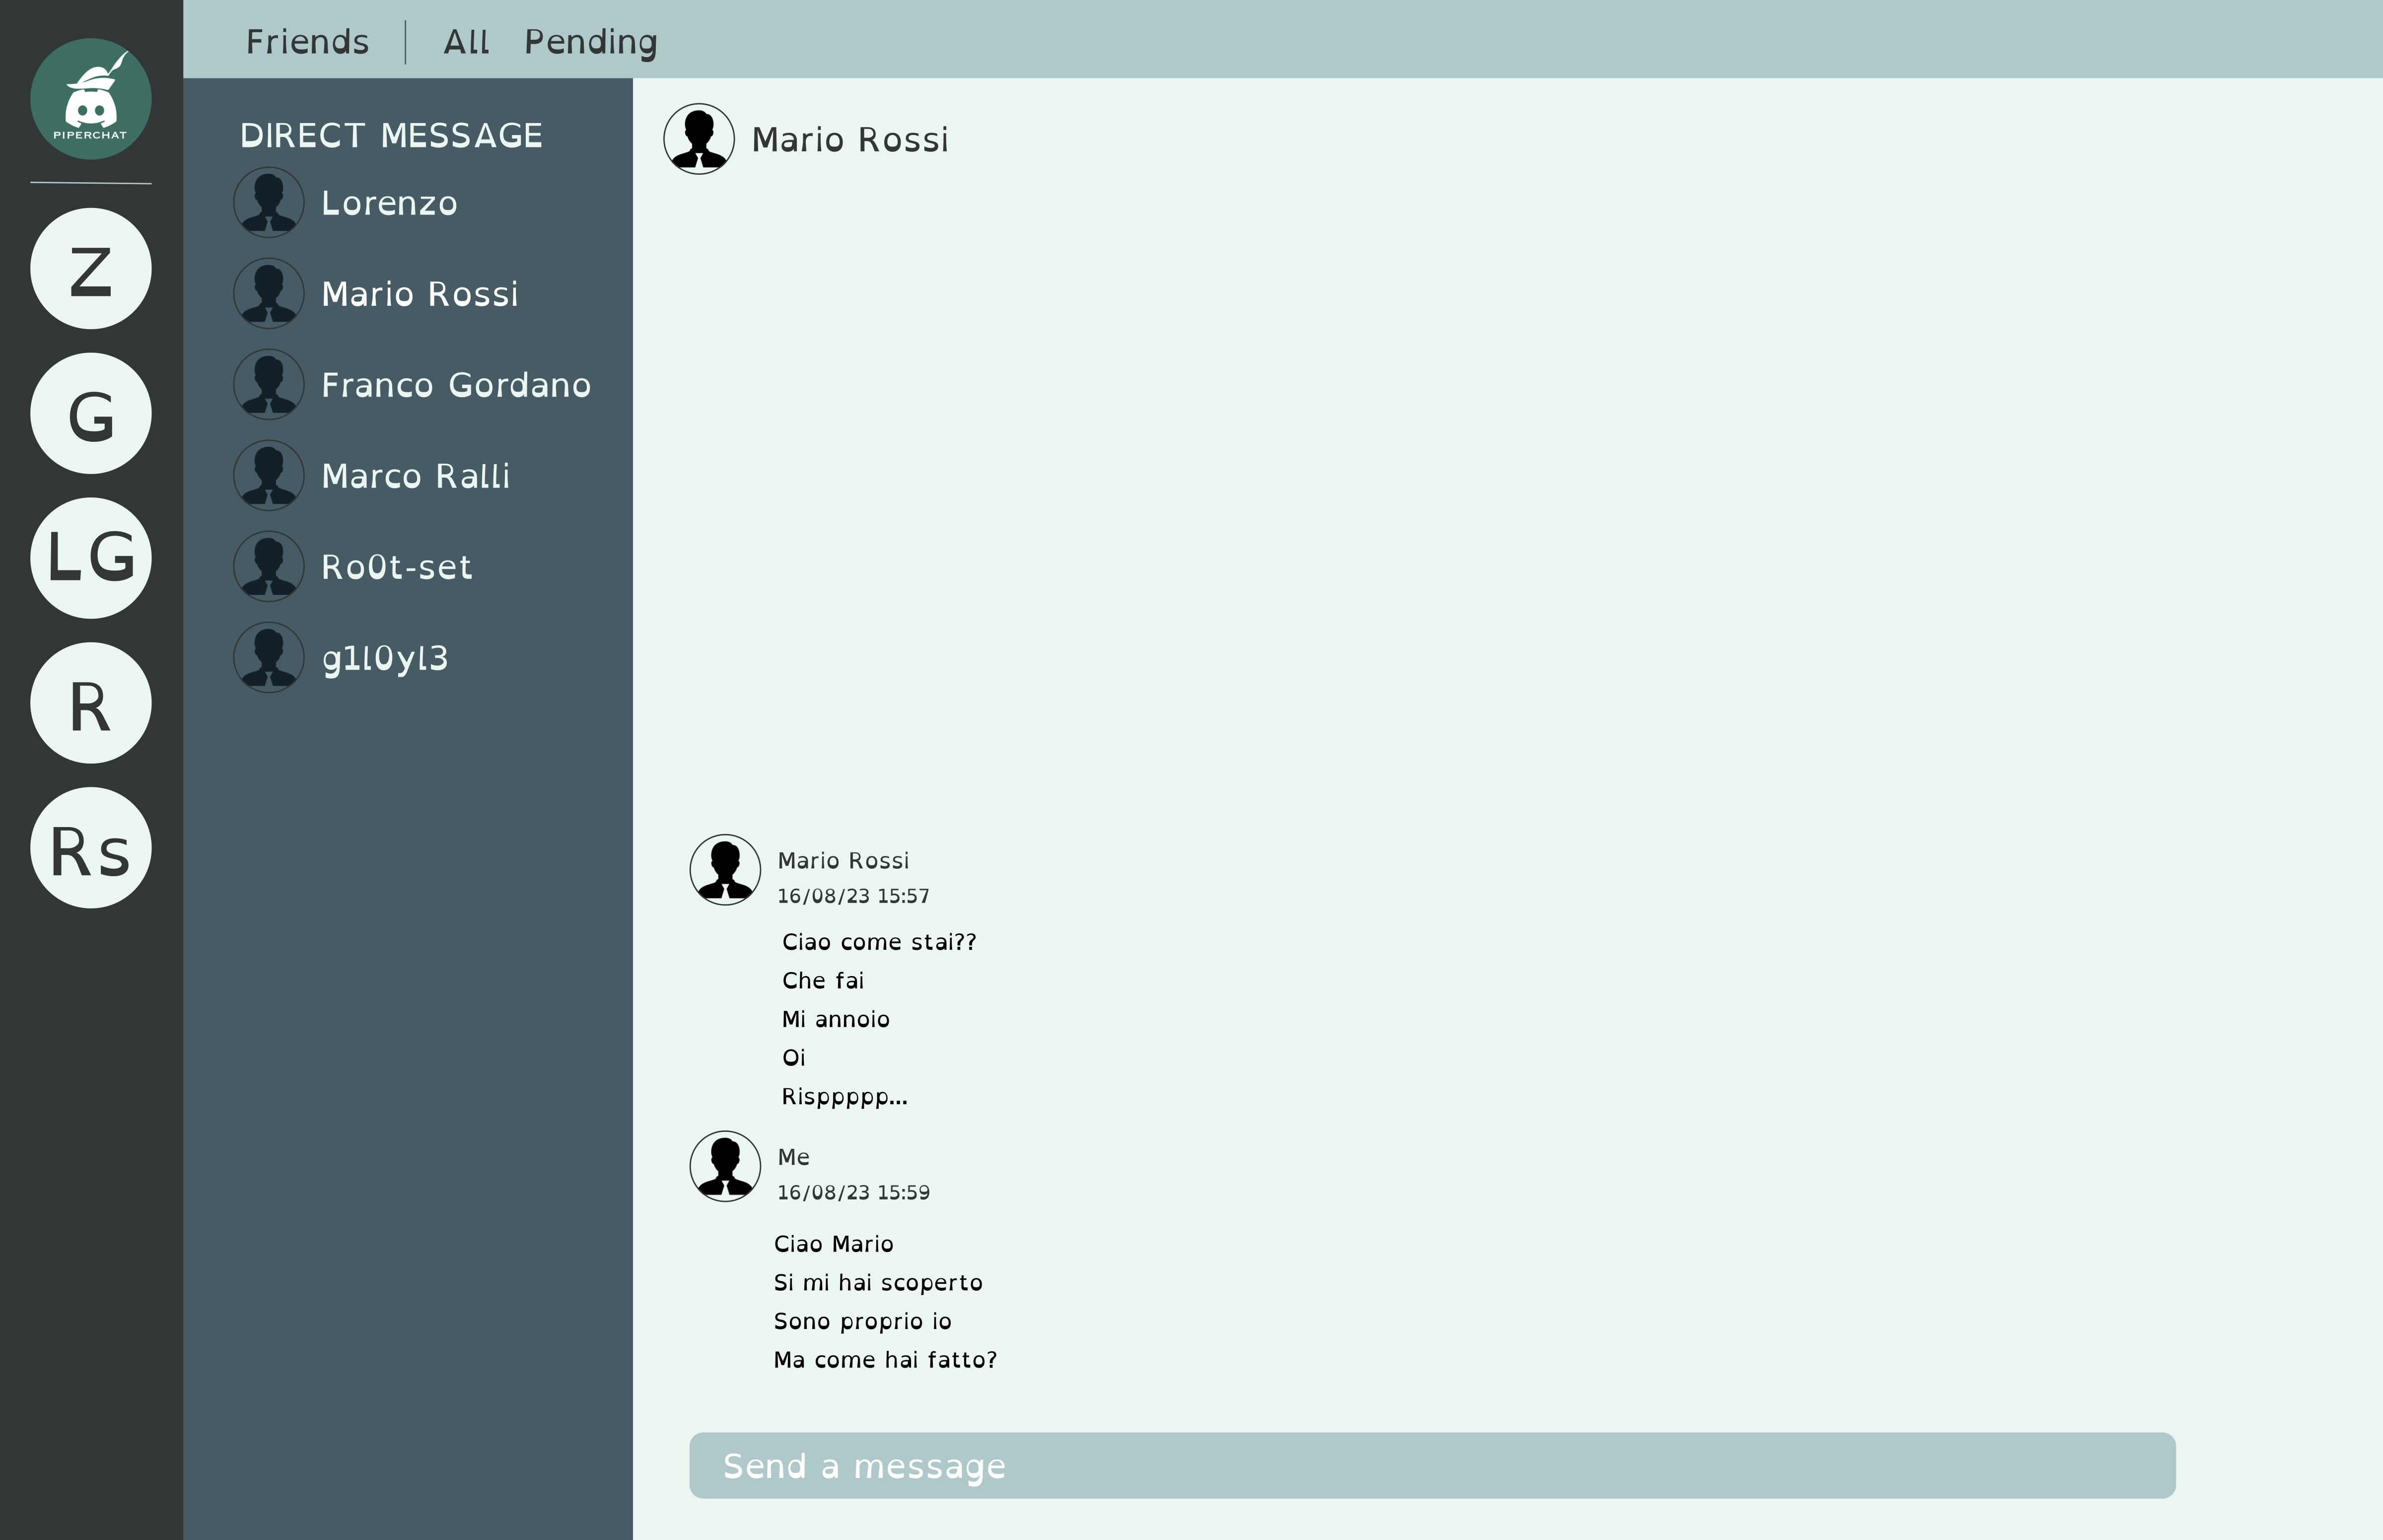
\includegraphics[angle=-90,width=0.92\textwidth]{img/mk2.jpg}
    \caption{Mockup chat}
    \label{fig:mockup2}
\end{figure}

\begin{figure}[htbp]
    \centering
    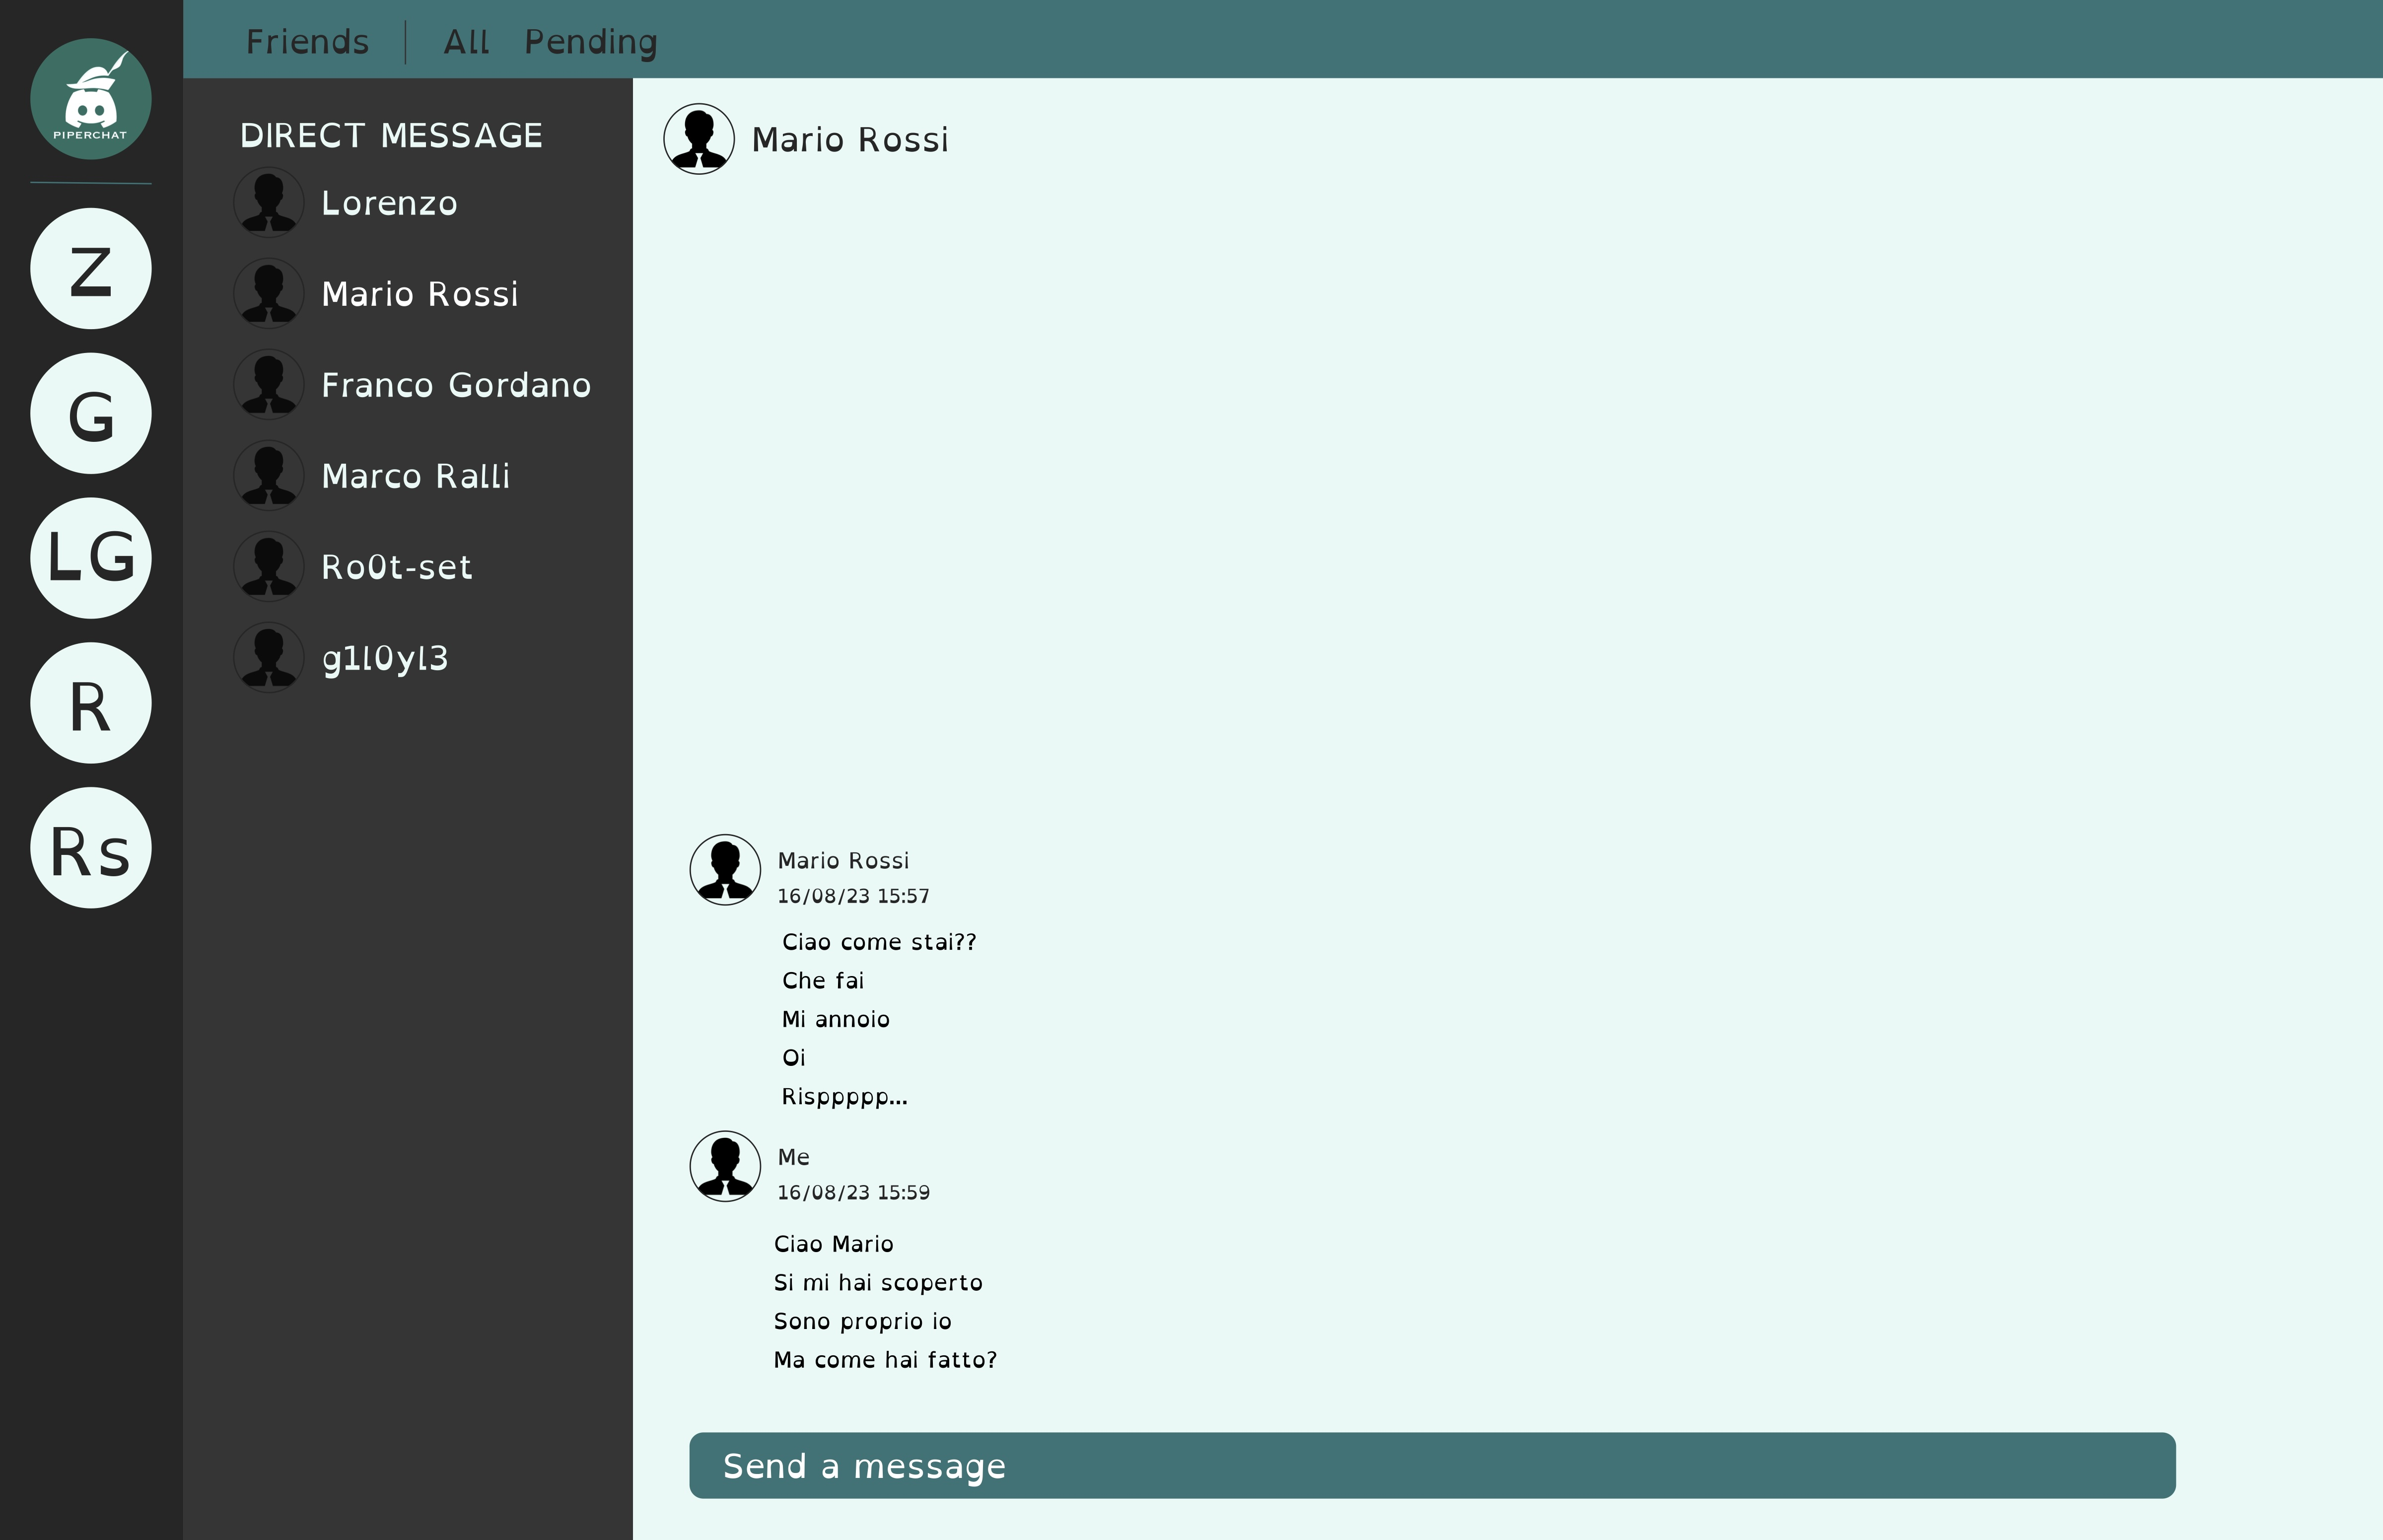
\includegraphics[angle=-90,width=0.92\textwidth]{img/mk3.jpg}
    \caption{Mockup chat con cambio dei colori}
    \label{fig:mockup3}
\end{figure}

\begin{figure}[htbp]
    \centering
    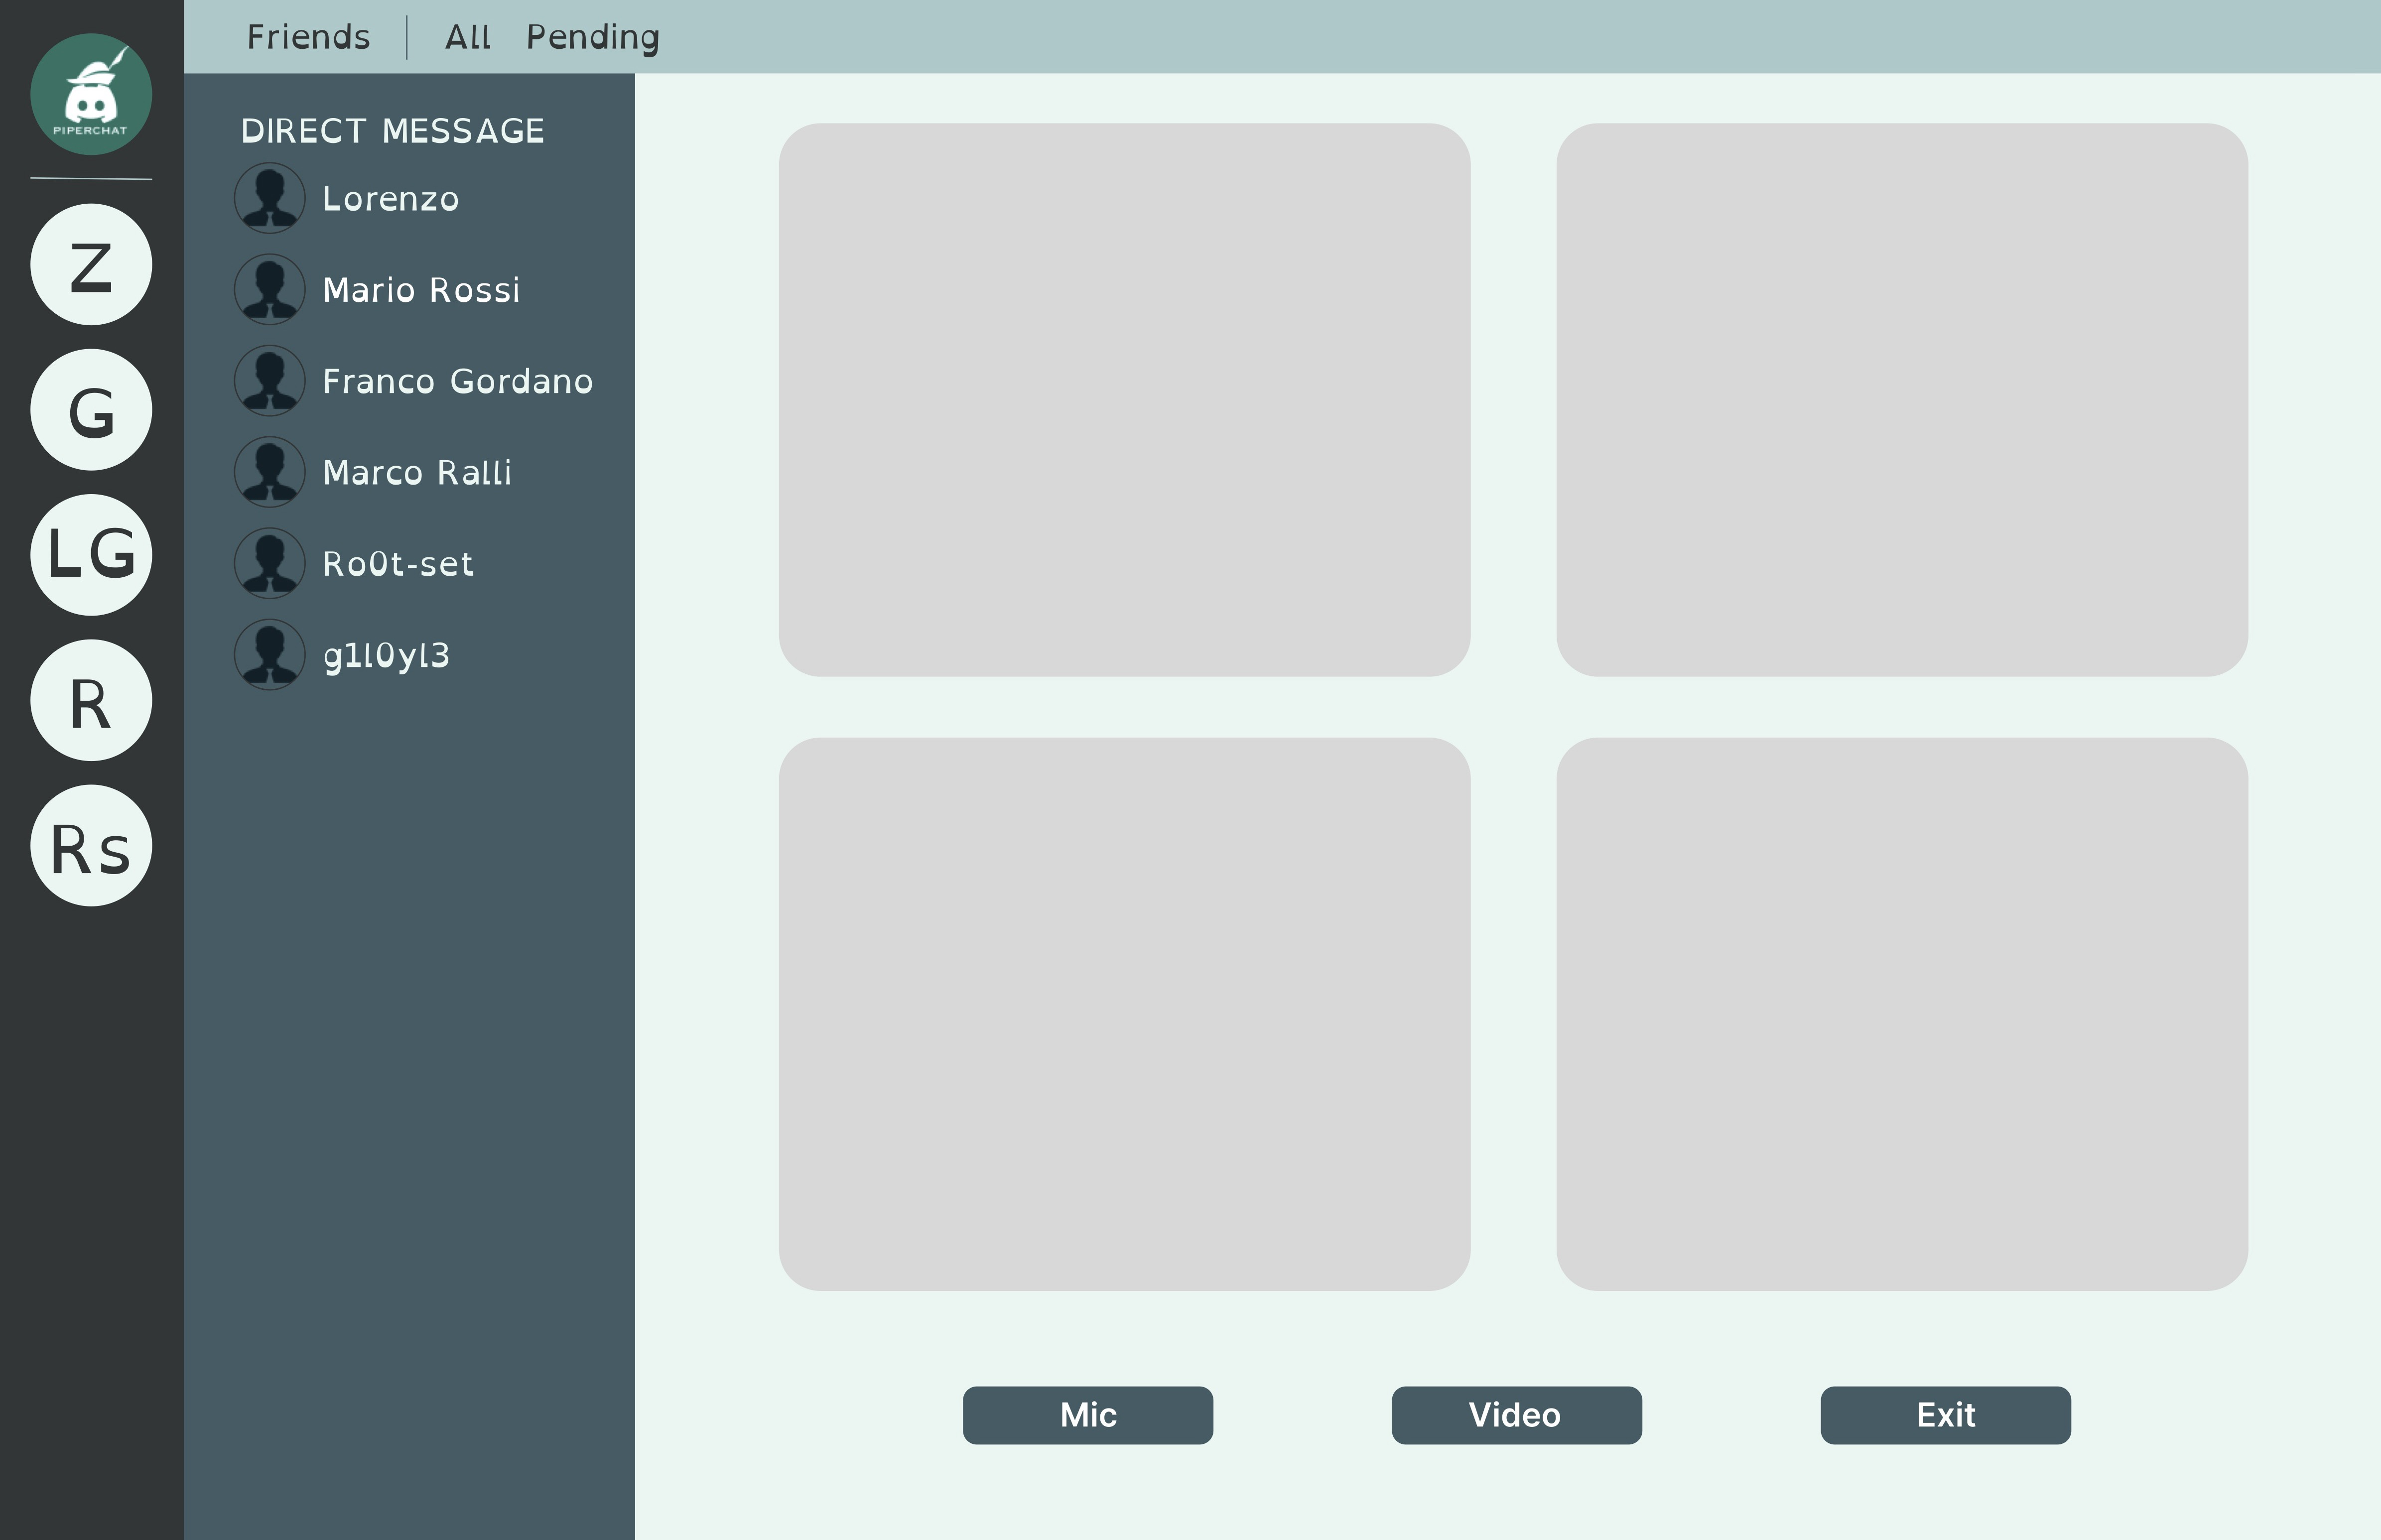
\includegraphics[angle=-90,width=0.92\textwidth]{img/mk4.jpg}
    \caption{Mockup video chat}
    \label{fig:mockup1}
\end{figure}

%
%
%
\newpage
\section{Design Architetturale}

Il sistema è realizzato mediante un'architettura a \emph{microservizi}.
%
Questo permette di suddividere la complessità in parti più piccole, ad alta coesione ed accoppiate in modo lasco.
%
Inoltre, ogni microservizio, se necessario, dispone di un \emph{database}, al quale può accedervi in modo esclusivo.

\begin{figure}[htbp]
    \centering
    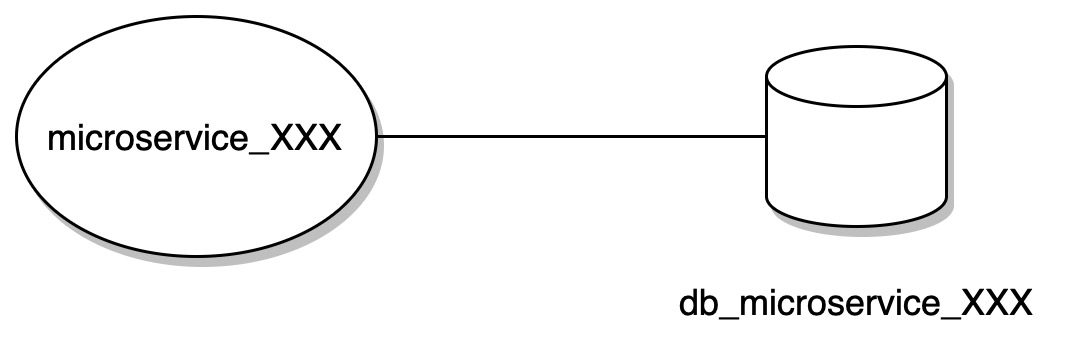
\includegraphics[width=\textwidth]{img/03-design/microservice-db.jpg}
    \caption{Un microservizio con il proprio database}
    \label{fig:microservice-db}
\end{figure}

A fronte di ciò sono stati identificati i seguenti microservizi:

\begin{itemize}
    \item \textbf{Notifications:} permette la gestione delle notifiche e lo status (online, ultimo accesso) degli utenti del sistema;

    \item \textbf{Users:} gestisce l'autenticazione degli utenti al sistema e tutti i dati relativi agli stessi. Inoltre, si occupa delle amicizie fra utenti;

    \item \textbf{Frontend:} fornisce l'accesso al sistema servendo la logica del client come Single Page Application;

    \item \textbf{Messages:} gestisce i messaggi degli utenti, sia nelle chat individuali, che per i canali testuali;

    \item \textbf{Monitoring:} permette il monitoraggio degli altri microservizi;

    \item \textbf{Piperchat:} gestisce la struttura di server e canali del sistema;

    \item \textbf{Webrtc:} gestisce tutto ciò che concerne \emph{WebRTC}, permettendo di istanziare video-chiamate all'interno del sistema.
\end{itemize}

%
%
%
\subsection{Comunicazione}

Al fine di permettere la comunicazione dei microservizi all'interno del sistema e permettere un'interazione con l'esterno, sono identificati i seguenti componenti:

\begin{itemize}
    \item \textbf{API Gateway:} componente che permette la comunicazione tra i client esterni al sistema, con i microservizi. Si occupa di redirezionare le richieste agli appositi servizi.

    \item \textbf{Broker:} componente che permette la comunicazione interna al sistema, fra i microservizi stessi.
\end{itemize}

\begin{figure}[htbp]
    \centering
    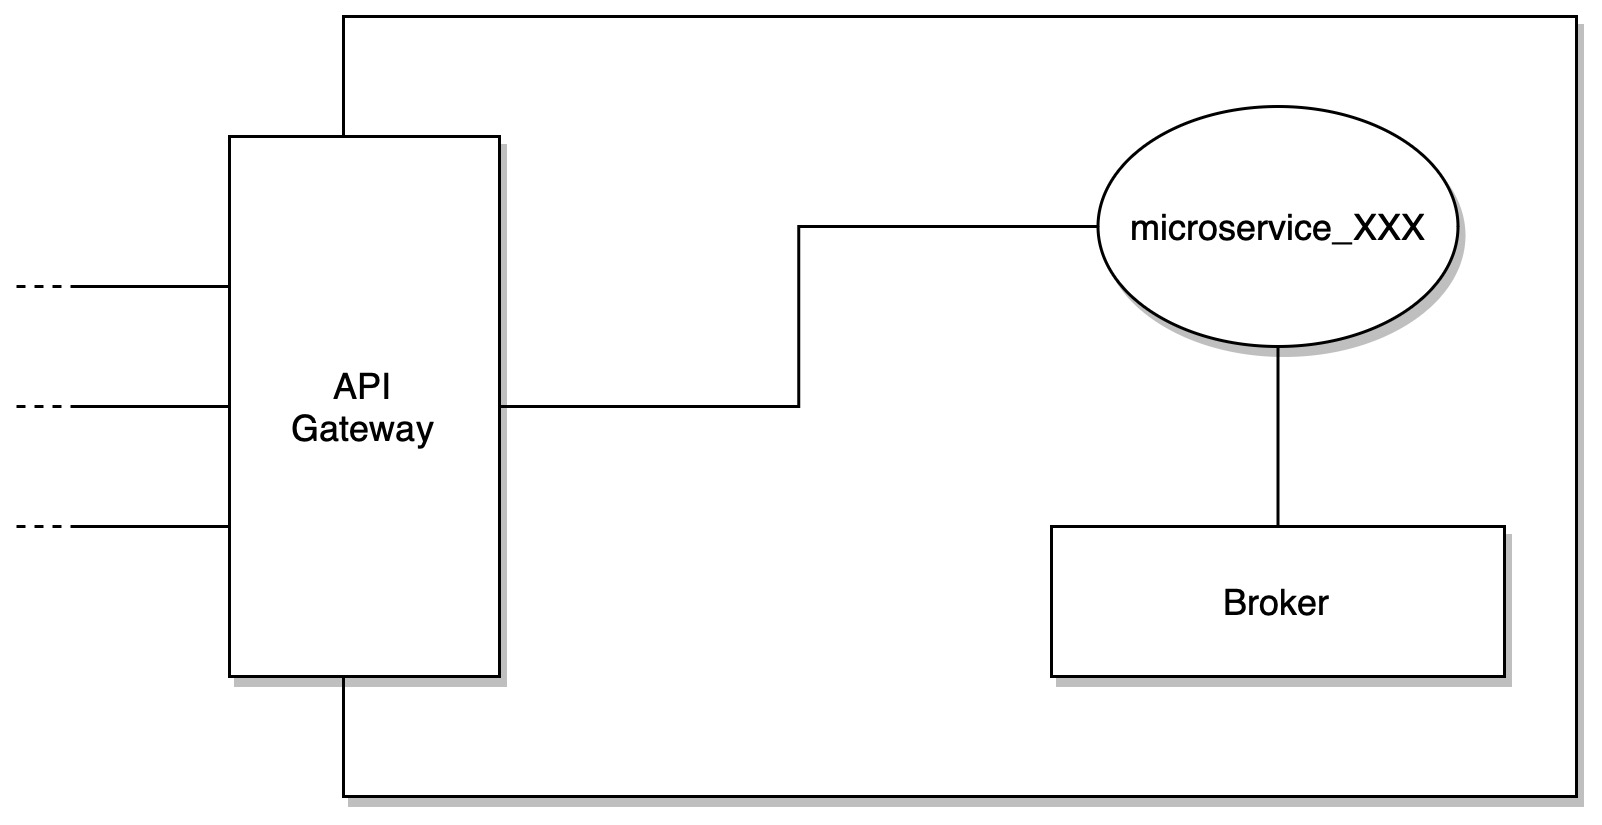
\includegraphics[width=\textwidth]{img/03-design/gateway-broker-microservice.jpg}
    \caption{Un microservizio collegato al Broker e all'API Gateway}
    \label{fig:gateway-broker-microservice}
\end{figure}

%
%
%
\subsection{L'architettura proposta}

Un utente, per accedere al servizio sfrutta l'\emph{API Gateway}.
In questo modo è possibile nascondere l'implementazione retrostante.

Di seguito è riportato lo schema architetturale del sistema.

\begin{figure}[htbp]
    \centering
    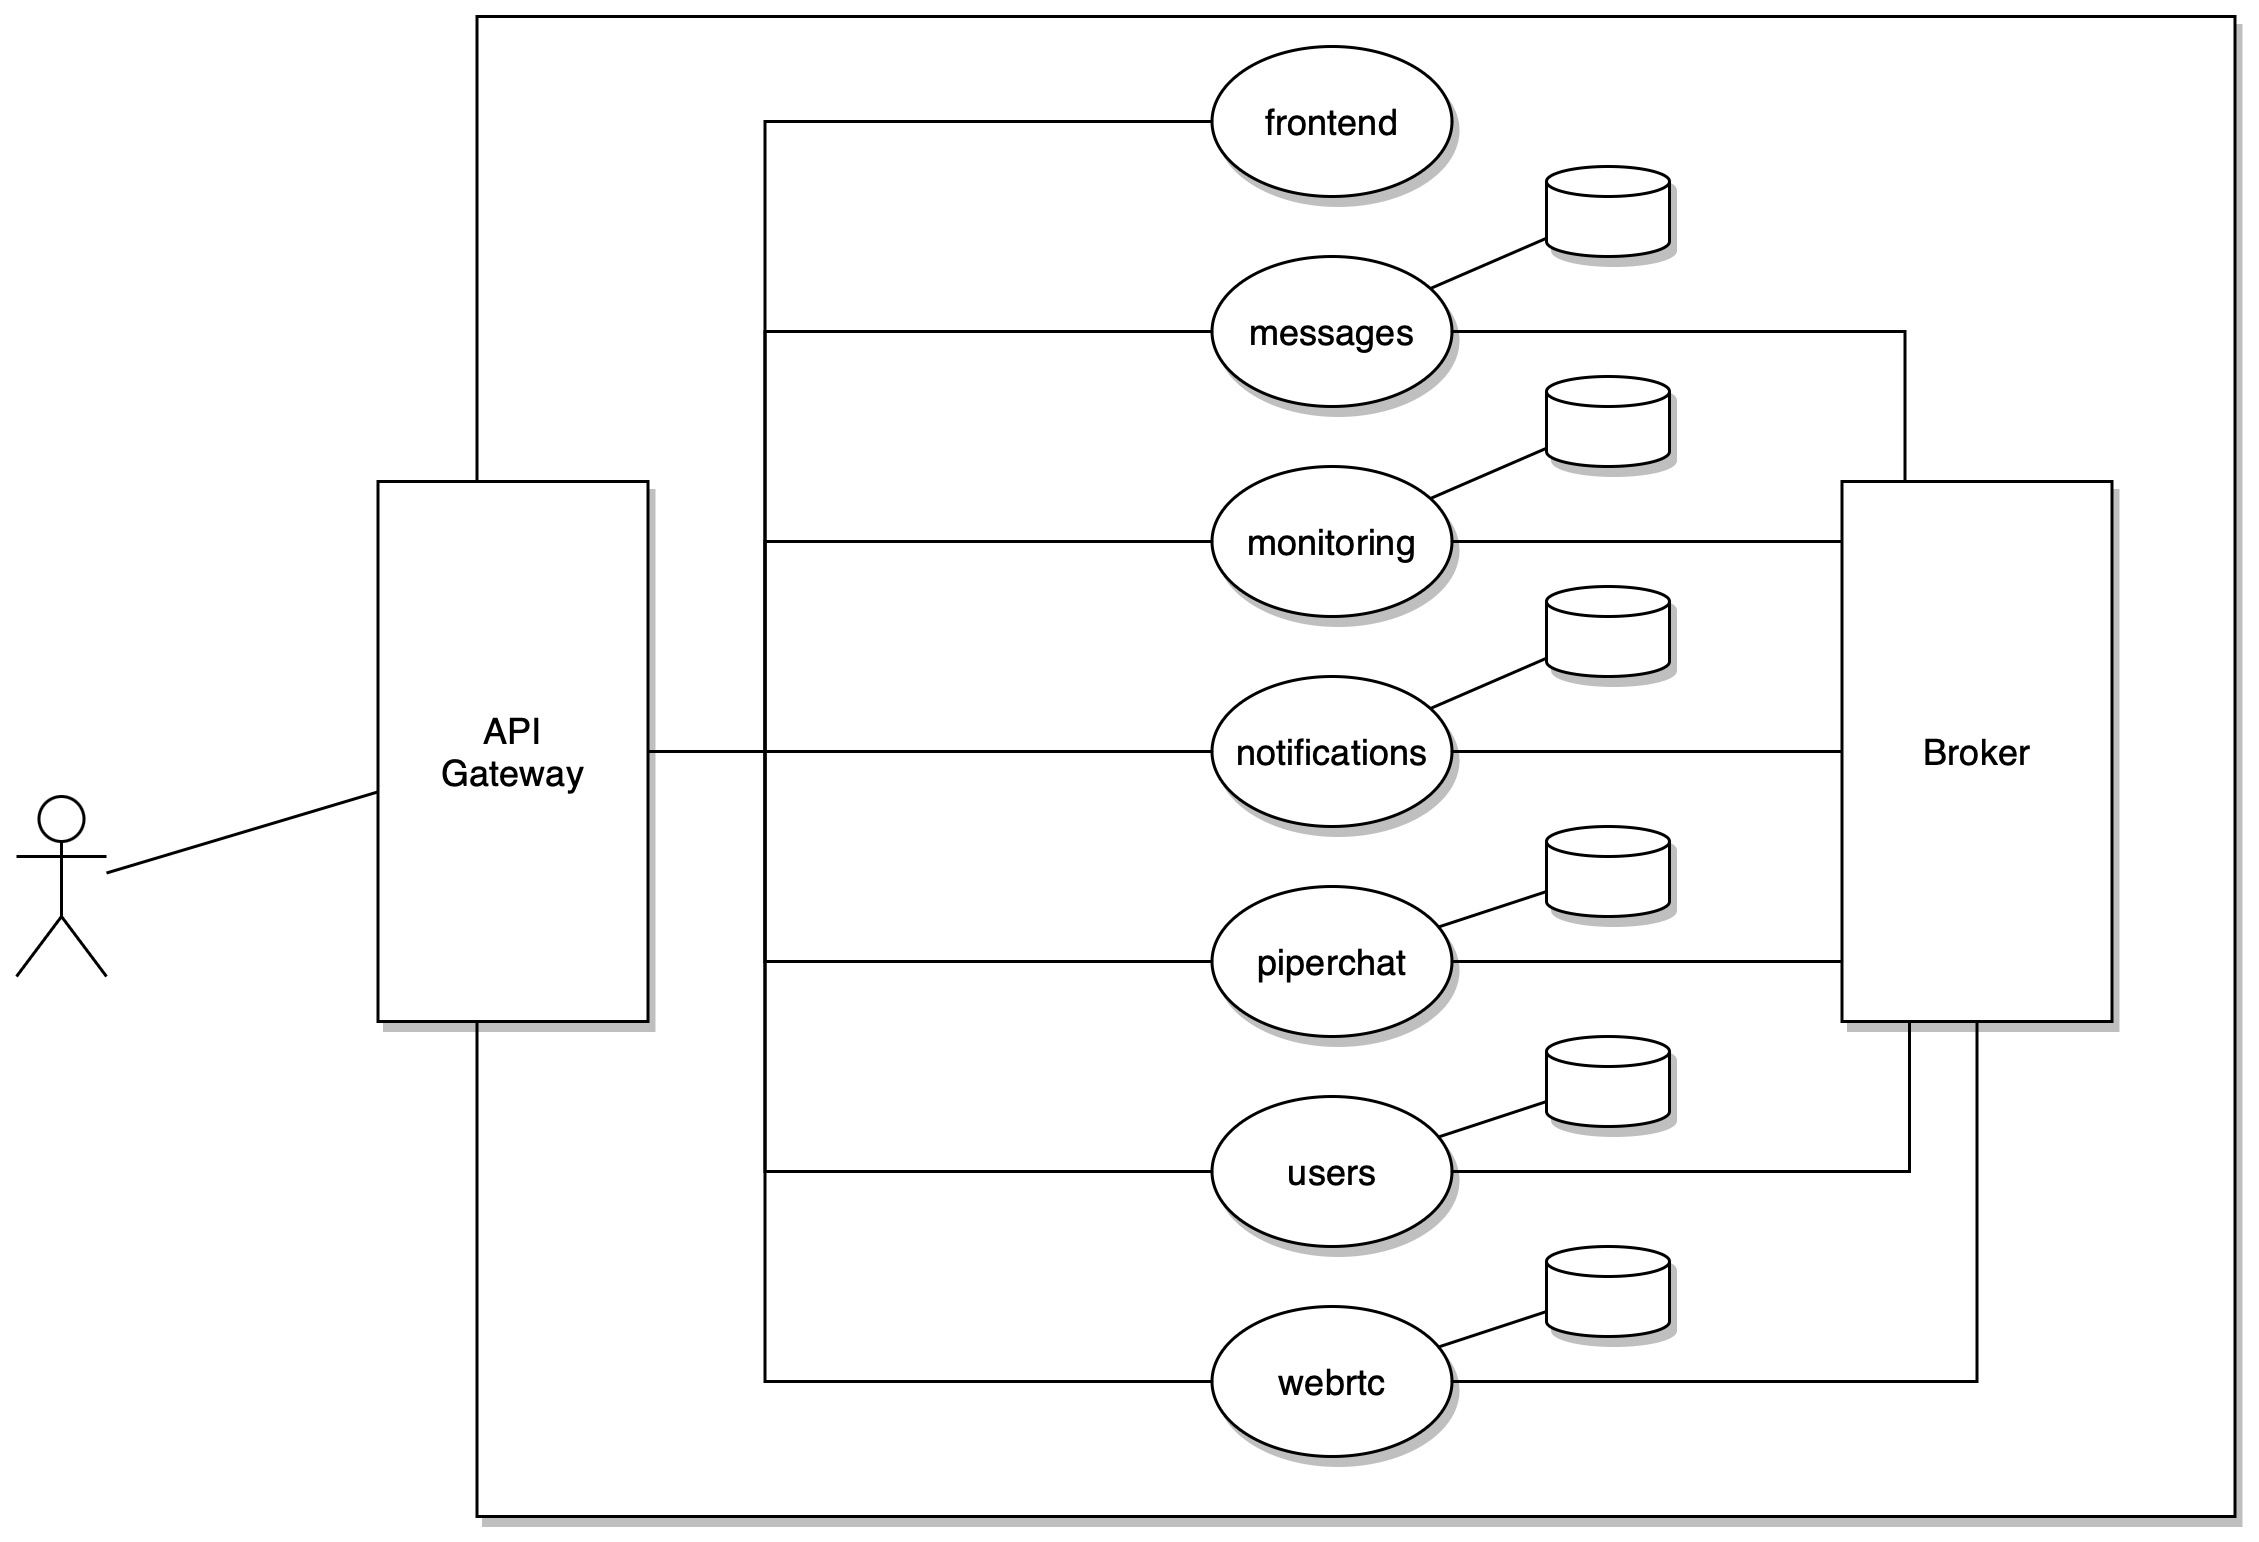
\includegraphics[angle=-90,width=0.95\textwidth]{img/03-design/architecture-schema.jpg}
    \caption{Architettura di Piperchat}
    \label{fig:piperchat-architecture}
\end{figure}
